\documentclass[handout]{beamer}

\usefonttheme[onlymath]{serif}

\setbeamertemplate{navigation symbols}{}
\usetheme{Berlin}
\setbeamertemplate{headline}{}
\defbeamertemplate*{footline}{Berlin} {
	\hbox{
		\begin{beamercolorbox}[wd=.1\paperwidth,leftskip=.3cm]{numbering}
			\insertframenumber{}$/$\inserttotalframenumber
		\end{beamercolorbox}
		\begin{beamercolorbox}[wd=.5\paperwidth,ht=2.5ex,dp=1.125ex]{author in head/foot}
			\hfill\insertshortauthor~~\insertshortinstitute
		\end{beamercolorbox}
		\begin{beamercolorbox}[wd=.4\paperwidth,leftskip=.3cm]{title in foot}
			\insertshorttitle
		\end{beamercolorbox}
	}
}

\usepackage[utf8]{inputenc}
\usepackage[T2A]{fontenc}
\usepackage[russian]{babel}
\usepackage{tikz}
\usepackage{ragged2e}
\usepackage{dsfont}
\usepackage[font=small,skip=0pt]{caption}

\usepackage{amsmath}
\usepackage{amsthm}
\usepackage{bm}
\usepackage{bbold}
\usepackage{subfigure}
\usepackage{multicol}
\usepackage{multirow}

\newtheorem{remark}{Замечание}

\title[Статистическое и машинное обучение]{Обучение с учителем. Классификация. Байесовский подход. Решающие деревья и ансамбли.}
\institute[ ]{%
	\small
	Санкт-Петербургский государственный университет\\
	Кафедра статистического моделирования
}
\date{}

\begin{document}
	
	\begin{frame}
		\titlepage
	\end{frame}

\begin{frame}{Обучение с учителем. Введение}

	{\bf Машинное обучение}~--- это раздел искусственного интеллекта, в котором разрабатываются методы и алгоритмы, позволяющие компьютерам обнаруживать закономерности в данных и делать прогнозы без явных инструкций.\bigskip
    % \textbf{Машинное обучение} позволяет извлекать закономерность из некоторого количества примеров.\\

	{\bf Пример задач}: 
	\begin{itemize}
		\item Регрессия: предсказание стоимости недвижимости, количества продаж некоторого товара, погоды.
		\item Классификация: предсказание ценовой категории товара, типа изображения, болеет ли человек или нет.
	\end{itemize}
\end{frame}

\begin{frame}{Обучение с учителем. Постановка задачи}
	
	{\bf Дано}: 
	\begin{itemize}
		\item Пространство объектов $\mathbb{X}$~--- множество описаний объектов (например, фотографии, тексты, таблицы с признаками).
		\item Пространство ответов $\mathbb{Y}$~-- множество меток или значений, которые нужно предсказывать (например, классы «кот»/«собака» или числовые значения цен).
	\end{itemize}	
	
	





	\textbf{Формализация задачи}: должна достигаться минимальная ошибка предсказания. \\
	Функционал ошибки $Q(\mathbf{X}, \mathbf{Y})$:\\
	\begin{tabular}{|l|l|}
	  \hline
	  Регрессия & Классификация \\
	  \hline
		 $\mathbb{E}||A(\xi)-\eta||^2_2$ & $\mathbb{E}||[(A(\xi)) \neq \eta]||_1$ \\
	   \hline
	\end{tabular}\\
	Для решения задачи необходимо определить:
	\begin{itemize}
		\item \textbf{Модель}. Пример: линейная регрессия (регрессия), SVM (классификация).
		\item \textbf{Функцию потерь и функционал ошибки}. Пример: MSE (регрессия), кросс-энтропия (классификация). 
		\item \textbf{Метод оптимизации}. Пример: стохастический градиентный спуск.
		\item \textbf{Гиперпараметры и метрики оценивания}: Пример: подбор гиперпараметров через GridSearch, MAPE (метрики регрессии), F1 score (метрики классификации).  
	\end{itemize}
\end{frame}

\begin{frame}{Классификация}
	В задаче классификации множество ответов $y_i$ дискретно.\\
	Рассмотрим линейный классификатор: 
	\begin{equation}
		A(x_i,w)=\mathsf{sign}(\sum_{j=1}^kw_jx_j + w_0).
	\end{equation}
	Множество ответов: $y_i \in \{+1, -1\}$. Линейный классификатор разделяет пространство на два класса. Будем считать, что среди $k$ признаков есть единичный.
	Функционал ошибки:
	\begin{equation}
		Q(\mathbf{X}, \mathbf{Y}) = \frac{1}{n}\sum_{i=1}^{n}[y_i\langle x_i, w\rangle < 0]=\frac{1}{n}\sum_{i=1}^{n}[M(x_i, y_i) < 0] \rightarrow \mathsf{min}_{w}
	\end{equation}
	$M(x_i, y_i)$ --- \textbf{величина отступа} (margin), абсолютная величина отступа говорит о степени уверенности классификатора. 
\end{frame}

\begin{frame}{Классификация}
	\small
	\textcolor{blue}{Проблема}: такой функционал нельзя минимизировать через градиентные методы.\\
	\textcolor{blue}{Решение}: можно минимизировать мажорирующий функционал.\\
	Ступенчатая функция потерь (ошибка на одном объекте) --- $[M < 0]$.
	\begin{figure}
	    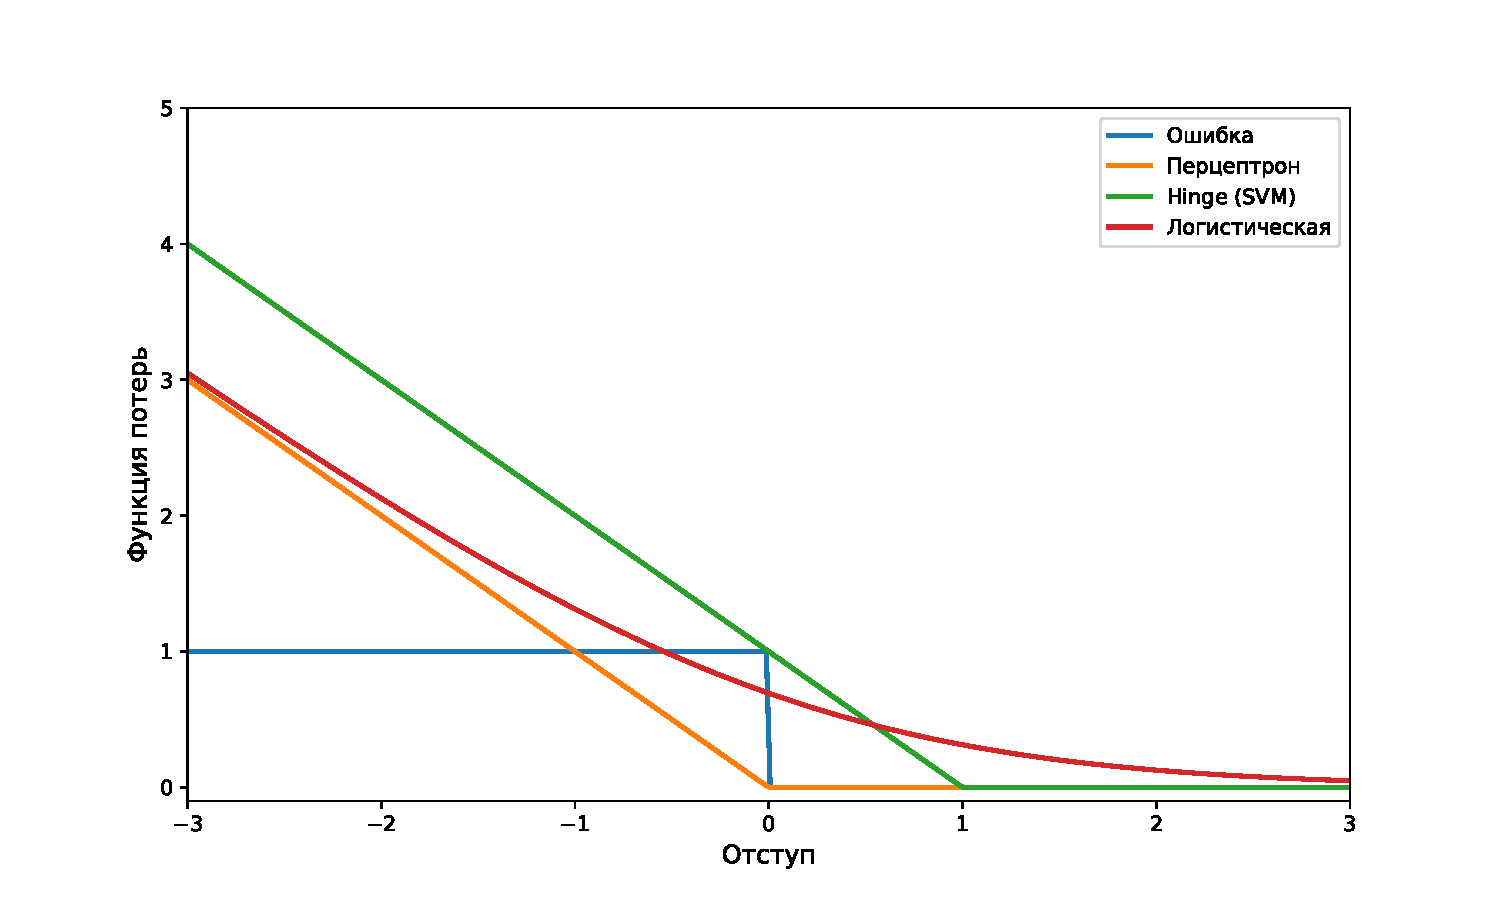
\includegraphics[scale = 0.63]{fig/loss_major.png}
	    \caption{\small Верхние оценки для пороговой функции потерь.
	    } 
	    \label{fig:w_series}
	\end{figure}

\end{frame}

\begin{frame}{Классификация: функции потерь}
	Различные функции потерь:
	\vspace*{5pt}
	\begin{enumerate}
		\item Логистическая: $L(M) = \mathsf{ln}(1+e^{-M})$
		\vspace*{5pt}
		\item Кусочно-линейная (SVM): $L(M) = \mathsf{max}(0, 1-M)$
\vspace*{5pt}
		\item  Кусочно-линейная (NN): $L(M) = \mathsf{max}(0, -M)$
\vspace*{5pt}
		\item Экспоненциальная: $L(M) = e^{-M}$
\vspace*{5pt}
		\item Сигмоидная: $L(M) = \frac{1}{1+e^M}$ (ANN - моделирование нейронных связей)
	\end{enumerate}
\end{frame}

\begin{frame}{Классификация: связь с модельным подходом}
	Рассмотрим логистическую регрессию: $L(M)= \mathsf{ln}(1+e^{-M})$.
	Логит:
	\begin{equation}
		z_i=\langle x_i, w\rangle = \mathsf{ln}\frac{p}{1 - p}, p = \frac{1}{1+e^{-\langle x_i, w\rangle}}=\sigma(\langle x_i, w\rangle)
	\end{equation}
	--- апостериорная вероятность. \\
	Функционал ошибки:
	\begin{equation*}
		Q(X, Y) = \sum_{i=1}^{n}\mathsf{ln}(1+e^{-y_i\langle x_i, w\rangle}) =
	\end{equation*}

	\begin{equation*}
 -\sum_{i=1}^n([y_i=1]\mathsf{ln}\frac{1}{1+e^{-z_i}}+[y_i=-1]\frac{1}{1+e^{z_i}})=
	\end{equation*}

	\begin{equation*}
	-\sum_{i=1}^n([y_i=1]\sigma(z_i)+[y_i=-1](1-\sigma(z_i))
	\end{equation*}
\end{frame}

\begin{frame}{Классификация: связь с модельным подходом}
	Применим модельный подход с распределением Бернулли (ММП). Метки классов $\{0, 1\}$.
	\begin{equation}
		p(y|X, w)=\Pi_{i=1}^np_i^{y_i}(1-p_i)^{1-y_i}.
	\end{equation} 
	Прологарифмируем.
	\begin{equation}
		 \sum_{i=1}^ny_i\mathsf{ln}(\sigma(\langle x_i, w\rangle)) + (1-y_i)\mathsf{ln}(1-\sigma(\langle x_i, w\rangle))
	\end{equation}
	Таким образом, ММП в данной задаче эквивалентен минимизации  функционала с логистической функцией потерь.
\end{frame}

\begin{frame}{Байесовский подход: общие понятия}
	\begin{enumerate}
		\item У нас есть выборка из случайной величины (например, сторона монетки).
		\item Мы хотим узнать распределение параметра $\theta$ (например, вероятность выпадения орла). Мы предполагаем, что он имеет некоторое \textbf{априорное} распределение. 
		\item Если применить полученные знания о выборке, то мы перейдем к \textbf{апостериорному} распределению.
	\end{enumerate}
	$p(\theta)$ --- \textbf{априорное} распределение параметра, $p(x|\theta)$ --- правдоподобие. Мы хотим узнать $p(\theta|x)$.\\
	\textbf{Апостериорное} распределение:
	\begin{equation}
		p(\theta|x) = \frac{p(x|\theta)p(\theta)}{p(x)}
	\end{equation}
\end{frame}

\begin{frame}{Байесовский подход: общие понятия}
	\begin{figure}
	    \includegraphics[scale = 0.5]{fig/b1.png}
	    \caption{\small Переход к апостериорному распределению.
	    } 
	    \label{fig:w_series}
	\end{figure}
\end{frame}

\begin{frame}{Байесовский подход: общие понятия}
	\begin{itemize}
		\item Частотный подход: "объективная неопределенность"
		\item Байесовский подход: "субъективное незнание"
	\end{itemize}
	Почему мы не можем всегда пользоваться частотным подходом (ММП)? $n$ должно быть большим.\\
	\textbf{Результатом} решения задачи в байесовском подходе является апостериорное распределение.\\
	Что дает байесовский подход?
	\begin{enumerate}
		\item \textbf{Регуляризация}. Мы получаем распределение, а не точечную оценку.
		\item Композитность: возможность объединить знания:
		\begin{equation*}
			p(y|x, z)=\frac{p(z|y)p(y|x)}{\int p(z|y)p(y|z)dz}
		\end{equation*}
		\item Инкрементальное получение результата.
	\end{enumerate}
\end{frame}

\begin{frame}{Байесовский подход: общие понятия}
	Формально: модель задается как параметрическое семейство распределений $\{\mathbb{P}_{\theta}|\theta\in\Theta\in\mathbb{R}^k\}$ с заданным на $\Theta$ априорным распределением $p(\theta)$.\\
	Каждый раз при получении новых данных мы обновляем наше апостериорное распределение.\\
	Пусть мы $m$ раз обновляли апостериорное распределение, получая данные $x_i$:
	\begin{equation*}
		p(\theta)\rightarrow p(\theta | x_1) \rightarrow \rightarrow p(\theta | x_1, x_2) \rightarrow \dots \rightarrow p(\theta | x_1, \dots, x_m)
	\end{equation*}
	Понятно, что $m$-ый шаг равносилен одному шагу с данными $x_1,\dots,x_m$.
\end{frame}

\begin{frame}{Байесовский подход: предел апостериорного распределения}
	Что будет происходить с апостериорным распределением, если будет поступать неограниченное количество данных?\\
	\begin{itemize}
		\item При выполнении \textit{условий регулярности}, апостериорное распределение $p(\theta |x_m)$ при $m \rightarrow \infty$ приближается к нормальному распределению $\mathcal{N}(\theta_0,(mI(\theta_0))^{-1})$.
		\item $\theta_0$ --- параметр истинного распределения, если распределение лежит в нашей модели.
		\item Если распределение не лежит в нашей модели, то $\theta_0$ минимизирует KL-расстояние от истинного распределения до нашей модели.
		\item $I(\theta_0)$ --- информация Фишера.  
	\end{itemize}
	Т.е. $p(\theta | x_m)$ стремится к вырожденному распределению в точке $\theta_0$.
\end{frame}

\begin{frame}{Байесовский подход: маргинальные распределения}
	Что если $\theta$ --- многомерный параметр?\\
	Пусть есть апостериорное распределение $p(\theta | x)$. По нему мы можем посчитать \textbf{маргинальное распределение} конкретной компоненты $\theta$ или группы компонент:
	\begin{equation*}
		p(\theta_i | x) = \int p(\theta | x)d\theta_{-i}
	\end{equation*}
	Такие интегралы часто приходится считать численно.
\end{frame}

\begin{frame}{Байесовский подход: как описать апостериорное распределение?}
	Мы по понятным причинам не можем полностью описать апостериорное распределение.\\
	Что тогда можно взять?
	\begin{enumerate}
		\item Точечные характеристики: среднее $\int \phi(\theta)p(\theta | x)d\theta$, максимум $\mathsf{argmax}_{\phi(\theta)}p(\theta | x)$.
		\item \textbf{Достоверный интервал} --- множество, в котором $\phi(\theta)$ лежит с опр. вероятностью.
	\end{enumerate}
\end{frame}

\begin{frame}{Байесовский подход: сопряженные распределения}
	Если данных много, то искать апостериорное распределение может быть затруднительно: $\int p(x | \theta)p(\theta)d\theta$ не считается аналитически для любых $p(x|\theta)$ и $p(\theta)$.\\
	Что делать в таком случае?\\
	\textbf{Сопряженное апостериорное распределение} --- распределение из параметрического семейства, для которого апостериорное распределение также в этом семействе.\\
	Таким образом, часто априорное распределение выбирают исходя из наличия сопряженного апостериорного.
\end{frame}

\begin{frame}{Байесовский подход: сопряженные распределения}
Примеры сопряженных распределений:

\begin{itemize}
	\item Бернулли - Гамма
	\item Биномиальное - Гамма
	\item Нормальное с изв. $\sigma^2$ - Нормальное (параметр $\mu$)
	\item Нормальное с изв. $\mu$ - Гамма (параметр $\sigma^2$)
\end{itemize}
Пример:
\begin{itemize}
	\item $X \sim B(\theta) \Rightarrow p(x_n | \theta) = \theta^{\sum x_i}(1-\theta)^{(n-\sum x_i)}$.
	\item Априорное распределение: $\theta \sim Beta(\alpha, \beta)$, $p(\theta)=\theta^{\alpha-1}(1-\theta)^{\beta - 1} / B(\alpha, \beta)$.
	\item $p(\theta | x_n)\propto \theta^{\sum x_i+\alpha-1}(1-\theta)^{n-\sum x_i+\beta-1}$
	\item Получаем, что $\theta|x_n \sim Beta(\alpha + \sum x_i, \beta + n - \sum x_i)$.
	\item \textcolor{red}{Трюк} с сопряженными распределениями: если будут новые данные, поместим их в параметры $Beta$!
\end{itemize}
\end{frame}

\begin{frame}{Байесовский подход: виды априорных распределений}
	\begin{itemize}
		\item \textbf{Неинформативные}: не несут дополнительной информации о значениях параметров (равномерные на $\theta$). Но: информация о том, что мы не можем предпочесть конкретное значение любому другому.
		\item \textbf{Информативные}: несут существенную дополнительную информацию о значениях параметра. Например: накопленные знания в некоторой предметной области. Если данных мало, то априорное распределение может ухудшить понимание.
		\item \textbf{Слабо информативные}: несут частичную информацию. Избавляемся от экстремальных значений. Что-то похожее на регуляризацию.
	\end{itemize}
\end{frame}

\begin{frame}{Байесовский подход: виды априорных распределений}
	\begin{figure}
	    \includegraphics[scale = 0.45]{fig/b2.png}
	    \caption{\small Априорные и апостериорные распределения.
	    } 
	    \label{fig:w_series}
	\end{figure}
\end{frame}

\begin{frame}{Байесовский подход: регрессия}
	Рассмотрим модель линейной регрессии:
	\begin{equation*}
		Y|\beta \sim \mathcal{N}(x\beta, \sigma^2I_n), \beta \sim \mathcal{N}(0, \sigma^2_0I_d).
	\end{equation*}
	Тогда 
	\begin{equation*}
		p(\beta|y) \propto \mathsf{exp}\{-\frac{1}{2\sigma^2}\sum(y_i-x_i\beta)\}exp\{-\frac{1}{2\sigma^2_0}\beta^T\beta\}.
	\end{equation*}
	Максимизация апостериорной плотности равносильна минимизации
	\begin{equation*}
		\sum(y_i-x_i\beta)^2+\frac{\sigma^2}{\sigma^2_0}\sum\beta^2_j.
	\end{equation*}
	Это же L2-регрессия с $\lambda=\frac{\sigma^2}{\sigma^2_0}$!
\end{frame}

\begin{frame}{Байесовский подход: предсказательное распределение}
	\begin{itemize}
		\item Пусть мы умеем считать $p(\theta | X)$.
		\item Тогда мы можем посчитать $p(X_{new}|\theta)$ --- \textbf{предсказательное распределение}.
	\end{itemize}
	\begin{equation*}
		p(X_{new}|\theta)=\int_{\theta}p(X_{new}, \theta|X)d\theta=\int_{\theta}p(X_{new}|\theta,X)p(\theta | X)d\theta
	\end{equation*}
	\begin{equation*}
		= \int_{\theta}p(X_{new}|\theta)p(\theta | X)d\theta
	\end{equation*}
	Проще сгенерировать данные:
	\begin{enumerate}
		\item Генерируем $\theta'$ из апостериорного распределения.
		\item Генерируем новое наблюдение $X_{new}$ из $p(*|\theta')$.
	\end{enumerate}
\end{frame}

\begin{frame}{Байесовский подход: оценка качества модели}
	В байесовском подходе вопрос "верна ли модель" не корректен --- модель не может быть полностью верна.\\
	Корректный вопрос: \textit{оказывают ли недостатки модели существенное влияние на выводы}?
	\begin{itemize}
		\item Если модель хорошая, то данные из предсказательного распределения должны быть похожи на реальные данные.
		\item Похожесть можно определять с помощью тестовых статистик $T$.
	\end{itemize}
	$P(T(X_{new}) > T(X)|X)$ --- \textbf{апостериорный предсказательный p-value}.
	\begin{itemize}
		\item Если апостериорный предсказательный p-value близок к $0$ или $1$, то качество модели низкое.
	\end{itemize}
\end{frame}

\begin{frame}{Байесовский подход: оценка качества модели}
	Как считать апостериорный предсказательный p-value?
	\begin{equation*}
		p=\int \int [T(X_{new}\geq T(X))]p(X_{new}|\theta)p(\theta|X)d(X_{new})d\theta
	\end{equation*}
	Как считают на самом деле:
	\begin{enumerate}
		\item Генерируют $K$ параметров $\theta'$ из апостериорного распределения.
		\item Для каждого из них генерируют $X_{new} \sim p(*|\theta')$.
		\item Для каждого $X_{new}$ считают $T(X_{new})$.
		\item Значение $p$ примерно равно доле $T(X_{new})$ больших $T(X)$.
	\end{enumerate}
\end{frame}

\begin{frame}{Байесовский подход: принятие решений}
	В байесовском подходе мы отходим от отвержения/не отвержения гипотезы в пользу \textbf{принятия решений}.
	\begin{itemize}
		\item Если не нужно принимать решение --- лучше оставить неопределенность в виде апостериорного распределения.
		\item Если принять решение все же нужно, то принимаем решение, учитывая риски.
	\end{itemize}
	Пусть есть набор решений $\delta_1, \dots, \delta_k$. \textbf{Риск} $R_i$ --- с.в., отражающая неопределенность последствий принятия решения $\delta_i$.\\
	После получения данных $X$ посчитаем \textbf{апостериорные риски} $R_i|X$ и выберем решение, минимизирующее \textbf{средний апостериорный риск} $E(R_i|X)$.
\end{frame}

\begin{frame}{Байесовский подход: классификация}
	Пример: классификация.\\
	\begin{itemize}
		\item Вероятностное пр-во $X\times Y$: $X$ --- объекты, $Y$ --- метки классов; известна плотность $p(x|y)p(y)$.
		\item Априорные вероятности $p(y)$ известны.
		\item Функции правдоподобия классов $p(x|y)$ известны.
		\item Решение --- выбор класса.
		\item Для каждой пары $(y, y')$ определен штраф $\lambda_{y,y'}$.

	\end{itemize}
\end{frame}

\begin{frame}{Байесовский подход: классификация}
	Риск для объекта $x$:
	\begin{equation*}
		R_{y'}=\sum_{y\in Y}\lambda_{y,y'}[Y|x=y].
	\end{equation*}

	Средний апостериорный риск:

	\begin{equation*}
		ER_{y'}=\sum_{y\in Y}\lambda_{y,y'}p(y|x)\propto\sum_{y\in Y}\lambda_{y,y'}p(x|y)p(y)
	\end{equation*}
	Т.е. Классификатор выглядит как:

	\begin{equation*}
		a(x)=\mathsf{argmin}_{y'}\sum_{y\in Y}\lambda_{y,y'}p(x|y)=
	\end{equation*}
\begin{equation*}
		\mathsf{argmin}_{y'}\sum_{y\in Y}\lambda_{y,y'}p(x|y)p(y)
	\end{equation*}
\end{frame}

\begin{frame}{Решающие деревья}
	Решающее дерево --- это бинарное дерево, которое строится следующим образом:
	\begin{enumerate}
		\item В корне дерева: выбирается признак и некоторый порог $t$, проверяется условие для каждого объекта $x_{ij} < t$. Если условие не выполняется, объект помещается в левый лист, иначе в правый (в случае категориального признака: проверка условия $x_{ij}=c$). Далее процедура повторяется в листах и т.д.
		\item Построение дерева \textit{прекращается} при достижении некоторых условий, например, некоторой глубины.
		\item \textit{Предсказание} decision tree --- некоторое отображение от выборки в листе, куда должен попасть новый объект, например, среднее значение или самый частый класс.
	\end{enumerate}
	Решающие деревья позволяют восстанавливать нелинейные зависимости произвольной сложности, применяются в задачах регрессии и классификации.
\end{frame}
	
\begin{frame}{Решающие деревья}
	\begin{figure}
	    \includegraphics[scale = 0.6]{fig/decision_tree.png}
	    \caption{\small Пример дерева решений.
	    } 
	    \label{fig:w_series}
	\end{figure}
\end{frame}

\begin{frame}{Решающие деревья}
	\begin{figure}
		    \includegraphics[scale = 0.7]{fig/decision_tree_ex1.png}
		    \caption{\small Пример классификации с decision tree.
		    } 
		    \label{fig:w_series}
	\end{figure}
\end{frame}

\begin{frame}{Решающие деревья: построение дерева}
	Как построить дерево, которое будет хорошо решать задачу регрессии или классификации?
	\begin{itemize}
		\item Можно построить дерево, которое имеет нулевую ошибку на любой выборке, но оно будет \textbf{переобученным}.
		\item Построение минимального решающего дерева с нулевой ошибкой --- NP полная задача.
	\end{itemize}
	Пусть имеется некоторый функционал ошибки $Q(X, j, t)$ для выборки в вершине, $j$ --- номер признака, $t$ --- некоторый порог; и некоторое условие останова.\\
	\textbf{Жадный алгоритм}:
	\begin{enumerate}
		\item На каждой итерации выполняется поиск $j, t$, которые минимизируют $Q(X, j, t)$. 
		\item Построение прекращается при выполнении условия останова. 
	\end{enumerate}
\end{frame}

\begin{frame}{Решающие деревья: построение дерева}
	После построения дерева можно произвести его стрижку (\textbf{prunning}) --- удаление некоторых вершин с целью повышения обобщательной способности.\\
	Какой функционал использовать для разбиения выборки в вершинах?
	\begin{equation}
		Q(R_m, j, s) = \frac{|R_l|}{|R_m|}H(R_l) + \frac{|R_r|}{|R_m|}H(R_r),
	\end{equation}
	где $H(R)$ --- \textbf{критерий информативности}, который оценивает качество распределения целевой переменной среди объектов $R$. Чем меньше разнообразие целевой переменной --- тем меньше значение критерия информативности.

\end{frame}

\begin{frame}{Решающие деревья: критерии информативности}
	Критерии информативности:
	\begin{itemize}
		\item Регрессия: $H(R) = \mathsf{min}_{c\in \mathbb{Y}}\frac{1}{|R|}\sum_{(x_i, y_i)\in R}(y_i - c)^2$
		\begin{equation*}
			H(R) = \frac{1}{|R|}\sum_{(x_i, y_i)\in R}\left(y_i-\frac{1}{|R|}\sum_{(x_j, y_j)\in R}y_j\right)^2
		\end{equation*}\\
		т.е. дисперсия в листе.
		\item Классификация: пусть $p_k=\frac{1}{|R|}\sum_{(x_i, y_i)\in R}[y_i=k]$. $\hat{k} = \mathsf{argmax}_{k}p_k$.
	\begin{equation*}
		H(R) = \mathsf{min}_{c\in\mathbb{Y}}\frac{1}{|R|}\sum_{(x_i, y_i)\in R}[y_i\neq c].
	\end{equation*}
	т.е. оптимальное предсказание --- $\hat{k}$. Следовательно, $H(R)=1-p_{\hat{k}}$.
	\end{itemize}
\end{frame}

\begin{frame}{Решающие деревья: критерии информативности}
	Критерии информативности:
	\begin{itemize}
		\item \textbf{Критерий Джини} (Jini impurity): пусть при классификации ответ в листе --- набор вероятностей. Качество такого набора можно измерить по \textbf{Brier score}:
		\begin{equation*}
			H(R) = \textsf{min}_{\sum_{k}c_k=1}\frac{1}{|R|}\sum_{(x_i, y_i)\in R}\sum_{k=1}^K(c_k-[y_i=k])^2. 
		\end{equation*}
		Оптимальный набор --- $\hat{c}=(p_1, \dots, p_K)$. Подставим этот набор и получим критерий Джини:
		\begin{equation*}
			H(R)=\sum_{k=1}^Kp_k(1-p_k)
		\end{equation*}
	\end{itemize}
\end{frame}

\begin{frame}{Решающие деревья: критерии информативности}
	Критерии информативности:
	\begin{itemize}
		\item \textbf{Энтропийный критерий}: рассматривается кросс-энтропия
		\begin{equation*}
			H(R) = \mathsf{min}_{\sum_kc_k=1}\left( -\frac{1}{|R|}\sum_{(x_i, y_i)\in R}\sum_{k=1}^K[y_i=k]\mathsf{ln}c_k\right).
		\end{equation*}
		После некоторых вычислений получаем, что оптимальный набор соотв. $p_i$. Энтропийный критерий:
		\begin{equation*}
			H(R)=-\sum_{k=1}^{K}p_k\mathsf{ln}p_k
		\end{equation*}
	\end{itemize}
\end{frame}

\begin{frame}{Решающие деревья: критерии информативности}
	\begin{figure}
	    \includegraphics[scale = 0.43]{fig/ic.png}
	    \caption{\small Критерии информативности.
	    } 
	    \label{fig:w_series}
	\end{figure}
\end{frame}

\begin{frame}{Решающие деревья: критерии останова}
	\begin{itemize}
		\item Ограничение максимальной глубины
		\item Ограничение минимального числа объектов в листе
		\item Ограничение максимального числа листьев
		\item Однородная выборка
		\item Минимальное улучшение функционала
	\end{itemize}
Преимущества decision tree:
	\begin{itemize}
		\item Интерпретируемость
		\item Простая обработка категориальных признаков
	\end{itemize}
	Недостатки:
	\begin{itemize}
		\item Сильно примитивнее других моделей.
	\end{itemize}
\end{frame}

\begin{frame}{Ансамбли}
	Обратимся к разложению ошибки на смещение и разброс (bias-variance tradeoff).\\
	\textbf{Bagging} --- метод, который позволяет уменьшить разброс модели. Этот метод обучает некоторое число алгоритмов так, что каждый алгоритм обучается на отдельных выборках, которые получены из исходной посредством бутстрапа.\\
	Разложение MSE в задаче регрессии:
	\begin{equation*}
		MSE=(\eta-\mathbb{E}\hat{\eta})^2 + \mathbb{E}(\mathbb{E}\hat{\eta} - \hat{\eta})^2
	\end{equation*}
	Разброс для ансамбля с усреднением, $\hat{\eta}=\frac{1}{M}\sum_{i=1}^M\hat{\eta}_i$:
	\begin{equation*}
		Var(\hat{\eta})=\frac{1}{M^2}\sum_{i=1}^MVar(\hat{\eta}_i)+\frac{1}{M^2}\sum_{i \neq j} Cov(\hat{\eta}_i, \hat{\eta}_j)
	\end{equation*}
\end{frame}

\begin{frame}{Ансамбли}
	Набор алгоритмов называется \textbf{ансамблем}, предсказание ансамбля в бэггинге:
	\begin{equation*}
		a_M(x)=\frac{1}{M}\sum_{m=1}^{M}b_m(x)
	\end{equation*}
	Смещение бэггинга совпадает со смещением базового алгоритма. При этом если базовые алгоритмы \textbf{некоррелированы}, то разброс уменьшается в $M$ раз.

\end{frame}

\begin{frame}{Random Forest}
	Модель \textbf{Random Forest} --- улучшение бэггинга решающих деревьев. Деревья становятся менее коррелированными благодаря тому, что при построении дерева в каждой вершине признак выбирается из случайного подмножества заданного размера $p$. Например, $p=\sqrt{d}$, где $d$ --- число признаков, для регрессии.\\
	Ограничения в построении дерева выбираются так, чтобы деревья получались глубокими --- такие деревья имеют низкое смещение.
\end{frame}

\begin{frame}{Gradient Boosting}
	\textbf{Бустинг} --- метод ансамблирования, в котором каждый добавляемый в композицию алгоритм обучается на ошибки ансамбля на предыдущем шаге.
	\textcolor{blue}{Пример}: Рассмотрим задачу регрессии
	\begin{equation}
		\frac{1}{2}\sum_{i=1}^{N}(a(x_i)-y_i)^2\rightarrow\mathsf{min}_a.
	\end{equation}
	Пусть предсказание алгоритма --- сумма предсказаний некоторых других базовых моделей:
	\begin{equation*}
		a_M(x)=\sum_{m=1}^Mb_{\theta_m, m}(x).
	\end{equation*}
	Построим первый базовый алгоритм:
	\begin{equation*}
		b_{\theta_1, 1}(x)=\mathsf{argmin}_{\theta}\frac{1}{2}\sum_{i=1}^N(b_{\theta}(x_i)-y_i)^2,
	\end{equation*}
\end{frame}

\begin{frame}{Gradient Boosting}
	Остатки:
	\begin{equation*}
		s_i^{(1)}=y_i-b_1(x_i).
	\end{equation*}
	Следующий алгоритм:
	\begin{equation*}
		b_{\theta_2,2}(x)=\mathsf{argmin}_{\theta}\frac{1}{2}\sum_{i=1}^N(b_{\theta}(x_i)-s_i^{(1)})^2.
	\end{equation*}
	И так далее. Заметим, что мы обучаемся на антиградиент:
	\begin{equation*}
		s_i^{(M)}=y_i-a_{M-1}(x_i)=-\frac{d}{dz}\frac{1}{2}(z-y_i)^2|_{z=a_{M-1}(x_i)}
	\end{equation*}
	Это базовая реализация бустинга.
\end{frame}

\begin{frame}{Gradient Boosting}
	Будем строить предсказание ансамбля как взвешенную сумму предсказаний базовых алгоритмов. Пусть имеется дифференцируемый функционал $L(y, z)$.
	\begin{equation*}
		a_M(x)=\sum_{m=0}^M\gamma_mb_{\theta_m, m}(x).
	\end{equation*}
	Как инициализировать значения?
	\begin{itemize}
		\item $b_0(x)=0$
		\item Классификация: $b_0(x) = \mathsf{argmax}_{y\in\mathbb{Y}}\sum_{i=1}^N[y_i=y]$
		\item Регрессия: $b_0(x) = \frac{1}{N}\sum_{i=1}^Ny_i$.
	\end{itemize}
	Добавление нового алгоритма в ансамбль:
	\begin{equation*}
		\sum_{i=1}^NL(y_i, a_{M-1}(x_i)+\gamma_Mb_{\theta_MM}(x_i))\rightarrow \mathsf{min}_{\theta_M, \gamma_M}.
	\end{equation*}
\end{frame}

\begin{frame}{Gradient Boosting}
	\textbf{Идея}: предсказание следующего алгоритма должно быть противоположно производной $L(y, z)$ в точке $z=a_{M-1}(x_i)$. Тогда вектор сдвигов совпадает с антиградиентом $L$.\\
	Таким образом, добавляя новый алгоритм, мы делаем шаг градиентного спуска.\\
	Рассмотрим задачу регрессии:
	\begin{equation*}
		b_{\theta_M, M}(x) = \mathsf{argmin}_{\theta}\sum_{i=1}^N(b_{\theta}(x_i) - y_i)^2.
	\end{equation*}
	После построения нового алгоритма, выбирается новый шаг:
	\begin{equation*}
		\gamma_M=\mathsf{argmin}_{\gamma\in\mathbb{R}}\sum_{i=1}^NL(y_i, a_{M-1}(x_i)+\gamma b_{\theta_M, M}(x_i)).
	\end{equation*}
	Описанный метод называется градиентным бустингом.
\end{frame}

\begin{frame}{Gradient Boosting: Регуляризация}
	\begin{itemize}
		\item Примитивные базовые алгоритмы плохо приближают антиградиент.
		\item Сложные базовые алгоритмы приведут к переобучению.
	\end{itemize}
	Решение этих проблем --- \textbf{сокращение шага}: вместо перехода в оптимальную точку делается укороченный шаг:
	\begin{equation*}
		a_M(x)=a_{M-1}(x)+\eta\gamma_Mb_{\theta_M, M}(x), \eta \in (0;1]
	\end{equation*}
	$\eta$ --- шаг обучения.\\
	Другое решение: стохастический градиентный бустинг.
	
\end{frame}

\begin{frame}{Gradient Boosting: Классификация}	
	Функция потерь для классификации:
	\begin{equation*}
		L(y, z)=\mathsf{ln}(1+e^{-yz}).
	\end{equation*}
	Тогда построение базового алгоритма:
	\begin{equation*}
		b_{\theta_M, M}=\mathsf{argmin}_{\theta}\sum_{i=1}^N\left( b_{\theta}(x_i) - \frac{y_i}{1+e^{y_ia_{M-1}(x_i)}}\right)^2.
	\end{equation*}
	Рассмотрим логистическую функцию потерь: 
	\begin{equation*}
	Q(a_M)=\sum_{i=1}^N\mathsf{ln}(1+e^{-y_ia_{M-1}(x_i)})e^{-y_i\gamma_Mb_{\theta_M, M}(x_i)}.
	\end{equation*}
Объекты с большим margin можно исключить.
\end{frame}

\begin{frame}{Gradient Boosting: Решающие деревья}
	Градиентный бустинг деревьев --- один из самых сильных методов машинного обучения.\\
	Представим предсказание решающего дерева в виде
	\begin{equation*}
		b_m(x)=\sum_{j=1}^{J_m}b_{mj}[x\in R_j],
	\end{equation*}
	где $j$ --- индекс листа, $R_j$ --- область разбиения, $b_{mj}$ --- ответ в листе.\\
	Предсказание ансамбля:
	\begin{equation*}
		a_M(x)=a_{M-1}(x)+\gamma_M\sum_{j=1}^{J_M}b_{M_j}[x\in R_j]=
	\end{equation*}
	\begin{equation*}
a_{M-1}(x)+\sum_{j=1}^{J_M}\gamma_Mb_{M_j}[x\in R_j].
	\end{equation*}

\end{frame}	

\begin{frame}{Gradient Boosting: Решающие деревья}
	Таким образом, добавление в ансамбль решающего дерева с $J_M$ листьями эквивалентно добавлению $J_M$ предикатов $x\in R_j$.\\
	Градиентный бустинг может лишь снизить смещение базовых моделей, а разброс бустинга не меньше разброса базового алгоритма.\\
	Поэтому в бустинге используются неглубокие решающие деревья, которые не склонны к переобучению.
\end{frame}

\begin{frame}{Gradient Boosting: AdaBoost}
	\textbf{AdaBoost}: используется экспоненциальная функция потерь $L(y, z)=e^{-yz}$.\\
	Метод сводит задачу поиска базового алгоритма к минимизации доли неверных ответов с весами при объектах.\\
	При использовании экспоненциальной функции потерь:
	\begin{equation*}
		s_i=y_ie^{-y_i\sum_{m=1}^{M-1}\gamma_mb_m(x_i)}=y_iw_i.
	\end{equation*}
	Что будет при наличии шумовых объектов? Отступ на них будет большой отрицательный, классификатор будет настраиваться исключительно на них.\\
	Теперь рассмотрим логистическую функцию потерь и получим:
	\begin{equation*}
		s_i=y_i\frac{1}{1+\mathsf{exp}(y_ia_{M-1}(x_i))}.
	\end{equation*}
	Шумовой объект будет иметь вес всего лишь в два раза больше.
\end{frame}

\begin{frame}{Gradient Boosting}
	Преимущества градиентного бустинга:
	\begin{itemize}
		\item Точнее многих архитектур.
		\item Быстро обучается.
		\item Хорошо работает с категориальными признаками.
		\item Множество хороших реализаций: XGBoost, CatBoost, LightGBM, с поддержкой Map Reduce.
	\end{itemize}
Недостатки:
\begin{itemize}
	\item Легко переобучается (Но: настройка patience, L1, L2 и т.д.)
	\end{itemize}
\end{frame}

\end{document} 